\def\myfiledate{2016-09-02}

\documentclass[a4paper,twoside]{article}
\usepackage{ucs}\usepackage[utf8x]{inputenc}
\usepackage{natbib}
\usepackage{chem}
%\usepackage{afterpage}
\usepackage{dirtree}

\usepackage{url}
\usepackage{color}
%\usepackage{multicol}
\usepackage{rotating} % loads graphicx
%\usepackage{longtable}
\usepackage{graphicx}
%\usepackage{verbatim}
\usepackage[pdftex,bookmarks=false,colorlinks]{hyperref}
\hypersetup{anchorcolor=black,citecolor=black,filecolor=black,linkcolor=black,%
  menucolor=black,urlcolor=black}
% "\pdfendlink ended up in different nesting level than \pdfstartlink"
% This happens when hyperref is used under pdftex and a citation splits
% across a page boundary. To fix it, note the page number of the error and
% specify the draft option to hyperref so you get an output PDF. Then you
% can see the citation in question and rewrite to fix it.

% activate to show "draft" watermark:
%\usepackage{draftwatermark}\SetWatermarkScale{5}

\oddsidemargin-5mm
\evensidemargin-5mm
\topmargin-15mm
\textheight250mm
\textwidth175mm
\raggedbottom
\parindent0mm
\parskip1.0ex plus0.5ex minus0.5ex

\renewcommand{\arraystretch}{1}
\renewcommand{\topfraction}{0.95}
\renewcommand{\dbltopfraction}{0.99}
\renewcommand{\bottomfraction}{0.99}
\renewcommand{\floatpagefraction}{0.95}
\renewcommand{\dblfloatpagefraction}{0.95}
\renewcommand{\textfraction}{0.2}
\setcounter{topnumber}{3}
\setcounter{dbltopnumber}{3}    % for 2-column pages
\setcounter{bottomnumber}{3}
\setcounter{totalnumber}{4}     % 2 may work better

\newcommand{\todo}[1]{{\color{red}\uppercase{\bf ((#1))}}}
\newcommand{\egcite}[1]{\citep[e.g.][]{#1}}

\newcommand{\tophline}{\hline\noalign{\vspace{1mm}}}
\newcommand{\middlehline}{\noalign{\vspace{1mm}}\hline\noalign{\vspace{1mm}}}
\newcommand{\bottomhline}{\noalign{\vspace{1mm}}\hline}

\def\nosep{\setlength\parsep{0mm}\setlength\topsep{0mm}\setlength\itemsep{0mm}}
\setlength{\columnsep}{8mm}

\def\mypageheader{Sander et al.: JVPP User Manual}
\markboth{\mypageheader}{\mypageheader}
\pagestyle{myheadings}
\sloppy

% this file was created automatically by njv, do not edit
\def\jvalversion{14.2}
 % \def\jvalversion{...}

% line break after \paragraph:
\makeatletter
\renewcommand\paragraph{\@startsection{paragraph}{4}{\z@}%
  {-2.0ex\@plus -1ex \@minus -.2ex}%
  {1.0ex \@plus .2ex}%
  {\normalfont\normalsize\bfseries}}
\makeatother

\begin{document}

\thispagestyle{empty}

\begin{center}

  \centering
\includegraphics[width=\textwidth]{spectrum}

  \vfill

  {\Huge\bf JVAL and JVPP User Manual}\\[3mm]

  {\Large The photolysis module JVAL-\jvalversion\\[2mm]
  The \underline{JV}AL \underline{P}re\underline{P}rocessor (JVPP)}

  \vfill

  {\LARGE\bf Rolf Sander et al.$^*$}\\[2mm]
  {\large Air Chemistry Department\\
  Max-Planck Institute of Chemistry\\
  PO Box 3060, 55020 Mainz, Germany\\
  \url{rolf.sander@mpic.de}}

  \vfill

  \tableofcontents

  \vfill

  {\large $^*$This manual is part of the electronic supplement of our
    article ``The photolysis module JVAL-\jvalversion, compatible with
    the MESSy standard, and the JVal PreProcessor (JVPP)'' by R.~Sander,
    P.~J\"ockel, O.~Kirner, A.~T.~Kunert, J.~Landgraf, and A.~Pozzer in
    Geosci.\ Model Dev.\ (2014), available at:
    \url{http://www.geosci-model-dev.net}}

  \vfill

  {\Large Date: \myfiledate}

  \vfill

  \centering
\includegraphics[width=\textwidth]{spectrum}

\end{center}

\twocolumn

\section{Introduction}

\citet{906} presented an efficient method for online calculations of
photolysis and heating rates which is based on parameterizations in 8
wavelength bands. This method is implemented in the JVAL code of the
MESSy system by \citet{2400}. Several calculations are necessary to
obtain the JVAL parameters based on UV/VIS spectra, quantum yields, and
their temperature and pressure dependencies. The JVal PreProcessor
(JVPP) was written to simplify this process. This manual describes how
to use JVPP and how to extend it for additional photolysis reactions.

\section{JVAL}

\subsection{Compiling and running the JVAL column model with the shell
  script {\tt xjval}}

First, go to the JVAL base directory:
\begin{verbatim}
cd jval
\end{verbatim}
Check that all settings in \verb|Makefile| are correct for the Fortran90
compiler on your system. If available, define the path of your netcdf
library in \verb|NETCDF_INCLUDE| and \verb|NETCDF_LIB|. If a netcdf
library is not available, set ``\verb|OUTPUT = ASCII|''. 

Next, use the tcsh script \verb|xjval| for compilation and execution of
the JVAL column model. Type:
\begin{verbatim}
./xjval
\end{verbatim}
The script will ask you if you want to compile the Fortran90 files and
then if you want to run the model. After successful completion, the
output will be in \verb|jval.nc| (or \verb|jval.dat| if \verb|ASCII|
output was chosen).

\subsection{The internal structure of JVAL}

The JVAL code consists of the Fortran90 files listed in
Tab.~\ref{tab:files_jval}. The call tree is shown in
Fig.~\ref{fig:calltree_jval}.

Note that for historical reasons, there are two variables for ozone in
the code: \code{relo3_2d} and \code{v3_2d}. Only \code{v3_2d} is used to
calculate $J$-values. The variable \code{relo3_2d} is used to calculate
heating rates (not discussed here).

\begin{table}
  \begin{center}
    \caption{Subdivision of the spectral range into 8 bands.
      $\lambda_{\rm ini}$ and $\lambda_{\rm fin}$ are the initial and
      final wavelength. $\lambda_i$ is a fixed wavelength inside each
      interval. Note that, for historical reasons, the bands are
      numbered from 0 to 7 in the JVAL code but 1 to 8 everywhere else.}
    \label{tab:eightbands}
    \begin{tabular}{lccccc}
      \middlehline
      number: name & 
      $\DS\frac{\lambda_{\rm ini}}{\mbox{nm}}$ & 
      $\DS\frac{\lambda_{\rm fin}}{\mbox{nm}}$ &
      $\DS\frac{\lambda_i}{\mbox{nm}}$\\
      \middlehline
      1: Schumann-Runge & 178.555 & 202.030 & \\
      2: Herzberg       & 202.030 & 240.970 & 205.1\\
      3: Hartley        & 240.970 & 289.870 & 287.9\\
      4:                & 289.870 & 305.500 & 302.0\\
      5: UV-B           & 305.500 & 313.500 & 309.0\\
      6:                & 313.500 & 337.500 & 320.0\\
      7: UV-A           & 337.500 & 422.500 & 370.0\\
      8: Chappuis       & 422.500 & 682.500 & 580.0\\
      \bottomhline
    \end{tabular}
  \end{center}
\end{table}

\begin{table*}[tbh]
  \begin{center}
    \caption{List of JVAL files}
    \label{tab:files_jval}
    \begin{tabular}{lp{0.55\textwidth}}
      \hline
      \multicolumn{2}{l}{\bf Fortran90 code}\\
      \hline
      \verb|jval.f90|                      & main column model file\\
      \verb|messy_cmn_photol_mem.f90|      & common definitions shared by different photolysis codes\\
      \verb|messy_jval.f90|                & static JVAL core file\\
      \verb|messy_jval_jvpp.inc|           & JVPP-generated file, included by \verb|messy_jval.f90|\\
      \verb|messy_main_blather.f90|        & message output utilities (generic MESSy submodel)\\
      \verb|messy_main_constants_mem.f90|  & physical constants (generic MESSy submodel)\\
      \verb|messy_main_tools.f90|          & miscellaneous tools (generic MESSy submodel)\\
      \verb|mo_netcdf.f90|                 & input/output\\
      \verb|mo_netcdf.f90-ascii|           & ASCII input/output\\
      \verb|mo_netcdf.f90-real|            & netCDF input/output\\
      \hline
      \multicolumn{2}{l}{\bf Other files and directories}\\
      \hline
      \verb|jval.nc|                       & output of JVAL\\
      \verb|jval.nml|                      & namelist file\\
      \verb|jvpp|                          & directory with JVPP code\\
      \verb|manual|                        & directory with JVAL manual\\
      \verb|xjval|                         & tcsh script to execute JVAL\\
      \hline
    \end{tabular}
  \end{center}
\end{table*}

\begin{figure*}[tbh]
  \framebox[\textwidth]{\begin{minipage}{0.9\textwidth}\dirtree{%
  .1 \code{PROGRAM jval}.
     .2 \code{jval_initialize}\DTcomment{intialization}.
        .3 \code{jval_read_nml_ctrl}\DTcomment{read {\tt\&CTRL} namelist}.
        .3 \code{aerosol_data}\DTcomment{initialise aerosol optical data \citep{2638}}.
     .2 \code{jval_init_memory}\DTcomment{allocate memory for arrays}.
     .2 \code{jval_physc}\DTcomment{main calculation}.
        .3 \code{jval_solar_time_control}\DTcomment{set solar cycle parameters}.
        .3 \code{jvalues}\DTcomment{calculate $J$-values}.
           .4 \code{column_cal}\DTcomment{calculate \chem{O_2} and
              \chem{O_3} column densities}.
           .4 \code{flux_cal}\DTcomment{calculate actinic fluxes}.
              .5 \code{slingo}\DTcomment{cloud particle radiative
                 properties \citep{2637}}.
              .5 \code{aero_2d}\DTcomment{apply humidity to aerosol data}.
              .5 \code{pifm}\DTcomment{practical improved flux method}.
                 .6 \code{pifmini}\DTcomment{pifm initialization}.
           .4 \code{jval_cal_uv}\DTcomment{calculate UV radiation}.
           .4 \code{jval_cal}\DTcomment{calculate all $J$-values in inc file}.
              .5 \code{jval_cal_*}\DTcomment{individual subroutines for
                 all species}.
     .2 \code{jval_result}\DTcomment{print results}.
     .2 \code{jval_free_memory}\DTcomment{deallocate memory of arrays}.
  }\end{minipage}}
  \caption{Call tree of the JVAL column model.}
  \label{fig:calltree_jval}
\end{figure*}

\subsection{Namelist control}

The file \verb|jval.nml| contains the coupling namelist \verb|&CPL| and
the control namelist \verb|&CTRL|. The coupling namelist is only needed
when JVAL is connected to a 3-dimensional base model via the MESSy
interface \citep{2400} but not for the column model. The variables in
\verb|&CPL| are:

\begin{description}
\item[\tt l\_skip\_lg:] JVAL has, in the Submodel Interface Layer
  (SMIL), an extension for tracers in Lagrangian representation (for the
  definition of representation, see \citet{2400}). If a tracer set
  \citep{2097} in Lagrangian representation is present, the J-values
  calculated in grid-point representaion are transformed to the
  Lagrangian representation for chemistry calculations along the
  trajectories. This can be switched off with {\tt l\_skip\_lg = T}. The
  default is {\tt F}, i.e., do not skip this calculation. This switch is
  only meaningful if a Lagrangian subsystem is running.
\item[\tt l\_force:] By default ({\tt l\_force = F}), only those
  J-values are calculated for which tracers in the selected chemical
  setup exist. This is done to avoid wasting CPU time. With this switch
  set to {\tt T}, the calculation of all J-values is forced. This is
  useful to compute all J-values diagnostically without any chemistry
  calculations.
\item[\tt l\_heating:] This switch (default: {\tt F}), if set to {\tt
    T}, enables the calculation of the UV heating rates by oxygen and
  ozone as additional diagnostic quantitites.
\item[\tt jval\_O3:] This variable contains two strings (channel name
  and object name, see \citet{2400}) which define the ozone input field.
  Examples are:
  \begin{itemize}
  \item \code{jval_O3 = 'tracer_gp', 'O3'}\\
    for an on-line coupling to the ozone tracer '\code{O3}', provided by
    the submodel TRACER in its channel '\code{tracer_gp}', or
  \item \code{jval_O3 = 'import_grid', 'O3clim'}\\
    for using an off-line prescribed ozone climatology '\code{O3clim}'
    provided by the submodel IMPORT\_GRID in its channel
    '\code{import_grid}'.
  \end{itemize}
\item[\tt jval\_cossza:] This defines the channel object providing the
  cosine of the solar zenith angle. For example,\\
  \code{jval_cossza = 'orbit', 'cossza'}\\
  selects the required values from object '\code{cossza}' provided by
  the submodel ORBIT via its channel '\code{orbit}'.
\item[\tt jval\_cdisse:] This defines the channel object providing the
  distance Sun-Earth (in AU), e.g.,\\
  \code{jval_cdisse = 'orbit', 'cdisse'}\\
  selects the required field from object '\code{cdisse}' provided by the
  submodel ORBIT via its channel '\code{orbit}'.
\item[\tt jval\_solar:] This defines the channel object providing
  information on the solar activity (solar cycle). If it is undefined
  (commented out in the namelist), the constant value {\tt r\_sol} in
  \verb|&CTRL| is used instead (see below). For example,\\
  \code{jval_solar = 'import_ts','solact'}\\
  selects the object '\code{solact}' from the channel '\code{import_ts}'
  of the submodel \code{IMPORT_TS}. The channel object can contain one
  of the following:
  \begin{itemize}
  \item The 10.7 cm solar radio flux in solar flux units (sfu,
    $10^{-22}$~\unit{W\,m^{−2}\,Hz^{−1}}) adjusted to the Sun-Earth
    distance of 1 AU: In this case a measure for the solar conditions
    between solar minimum (0, corresponding to about 70 sfu
    \citep{3016}) and solar maximum (1, corresponding to 270 sfu) is
    linearly interpolated for the actual 10.7cm flux and applied as
    solar cycle modulation of the J-value calculations.
  \item 16 parameters (all adjusted to a Sun-Earth distance of 1 AU):
    \begin{description}
    \item[1:] Lyman-$\alpha$ total flux at the top of the atmosphere
      (\code{phi_la}), e.g., 3\E{11} for a low solar activity
      \citep{2633}.
    \item[2:] Integrated flux over the Schumann-Runge bands (interval 1)
      at the top of the atmosphere (\code{SR_toa_flux}).
    \item[3-9:] Flux at the top of the atmosphere at the fixed
      wavelengths $\lambda_i$ inside intervals 2-8 taken from
      Table~\ref{tab:eightbands} (\code{flux}).
    \item[10-16:] For each of the intervals, the ratio of the integrated
      flux (from $\lambda_{\rm ini}$ to $\lambda_{\rm fin}$, see
      Table~\ref{tab:eightbands}) to the flux at the fixed wavelength
      $\lambda_i$ (\code{f0}).
    \end{description}
    The unit of \code{phi_la}, \code{SR_toa_flux}, and \code{flux} must
    be \unit{\mbox{photons}\,cm^{-2}\,s^{-1}}.
  \end{itemize}

\end{description}

The variables in \verb|&CTRL| are:

\begin{description}
\item[\tt r\_sol:] For the solar cycle, a value of 0 defines the solar
  minimum, and a value of 1 the solar maximum. This variable is
  overwritten if {\tt jval\_solar} in \verb|&CPL| is set.
\item[\tt qy\_ch3coch3:] There are three options to calculate the
  quantum yield for acetone (\chem{CH_3COCH_3}) photolysis, based on
  different publications. For details, see
  \code{jvpp/dat_lit/hardcoded/jval_cal_CH3COCH3.f90}.
\end{description}

Normally, there is no need to change the default settings of the
namelists.

\begin{figure*}[tbh]
  \begin{center}
  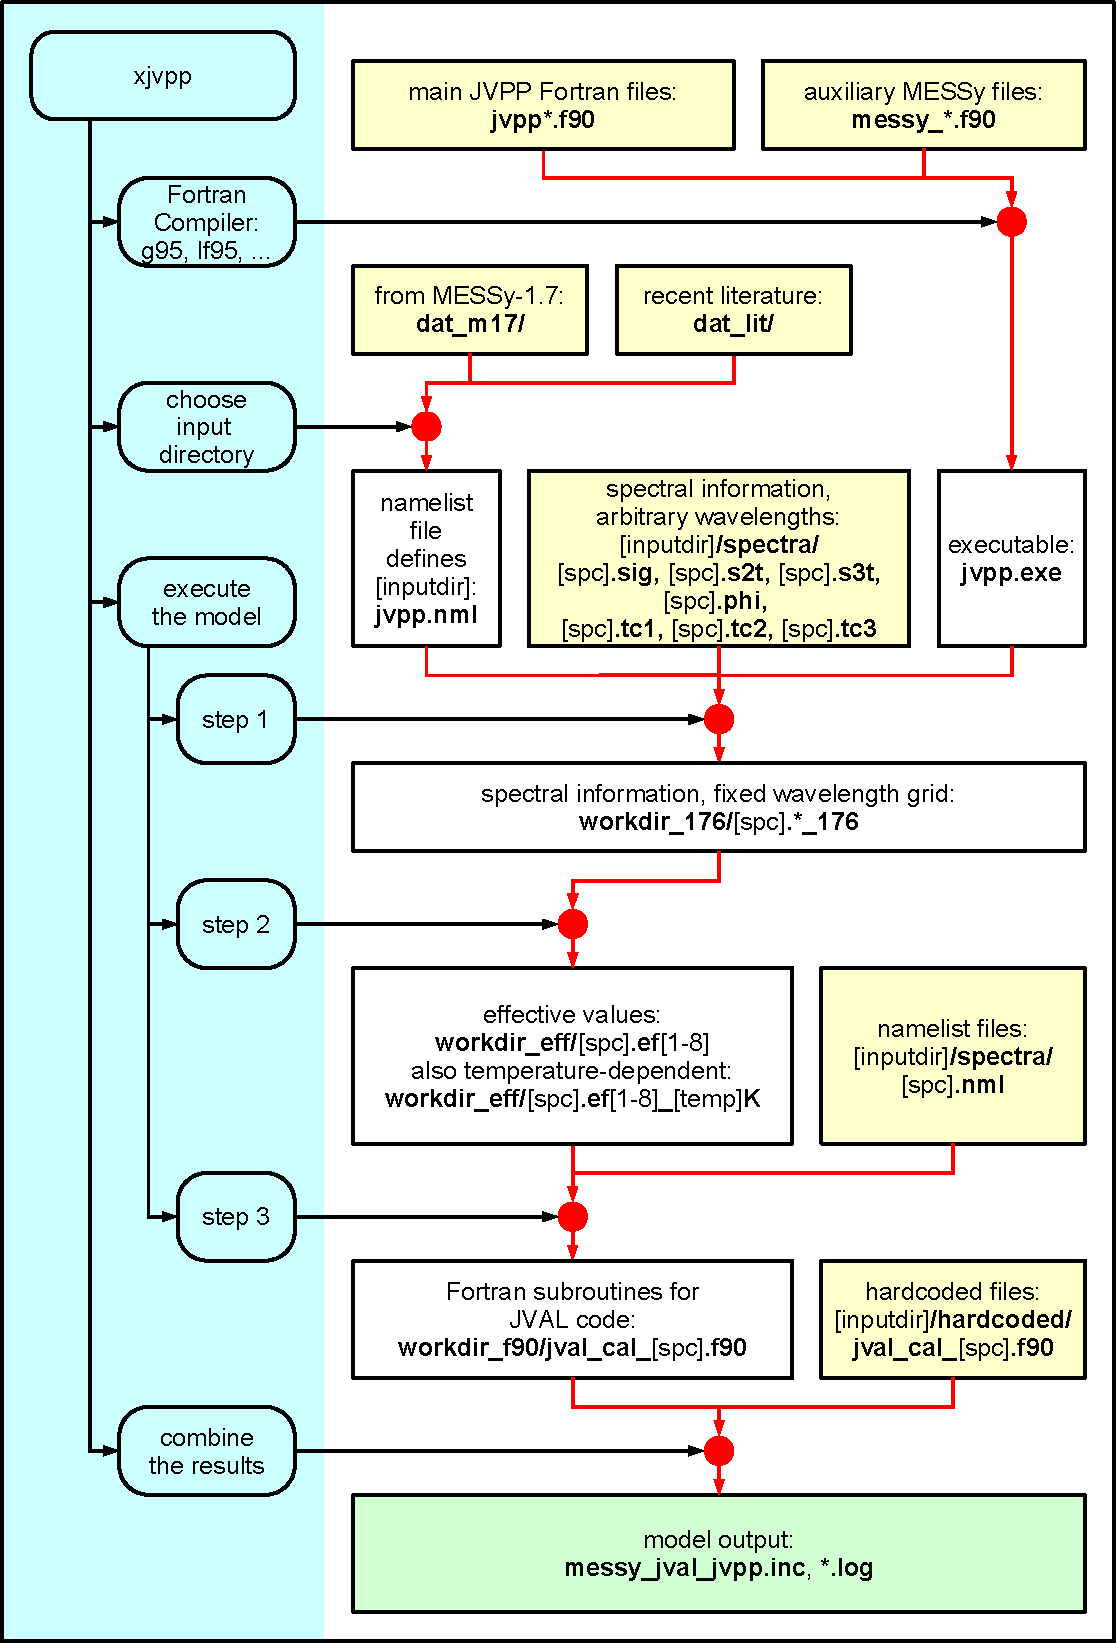
\includegraphics[width=0.84\textwidth]{flowcontrol_xjvpp}
  \end{center}
  \caption{Illustration of the tasks performed by {\tt xjvpp}. {\tt
      xjvpp} and all scripts called by {\tt xjvpp} are shown on a blue
    background. User-generated (static) input files are shown on a
    yellow background whereas automatically generated temporary files
    are shown on a white background.}
  \label{fig:flowcontrol_xjvpp}
\end{figure*}

\begin{table*}[tbh]
  \begin{center}
    \caption{List of JVPP files}
    \label{tab:files_jvpp}
    \begin{tabular}{lp{0.55\textwidth}}
      \hline
      \multicolumn{2}{l}{\bf Fortran90 code}\\
      \hline
      \verb|jvpp.f90|                      & main program\\
      \verb|jvpp_step1.f90|                & step 1 (see text)\\
      \verb|jvpp_step2.f90|                & step 2 (see text)\\
      \verb|jvpp_step3.f90|                & step 3 (see text)\\
      \verb|jvpp_mem.f90|                  & common variable declarations\\
      \verb|messy_cmn_photol_mem.f90|      & common definitions shared by different photolysis codes\\
      \verb|messy_main_constants_mem.f90|  & physical constants\\
      \verb|messy_main_math_lsq.f90|       & least-square fit methods\\
      \verb|messy_main_math_spline.f90|    & spline methods\\
      \hline
      \multicolumn{2}{l}{\bf Input}\\
      \hline
      \verb|cheb_coeff.txt|                & Chebyshev coefficients (for \chem{O_2} cross sections)\\
      \verb|jvpp.nml|                      & automatically created namelist file\\
      \verb|dat_m17/|                      & obsolete data from MESSy-1.7\\
      \verb|dat_lit/|                      & data from recent literature\\
      \verb|dat_lit/spectra/*.nml|         & individual namelist files\\
      \verb|dat_lit/spectra/*.sig|         & original spectra, as from the literature\\
      \verb|dat_lit/spectra/*.s2t|         & spectra at 2 temperatures\\
      \verb|dat_lit/spectra/*.s3t|         & spectra at 3 temperatures\\
      \verb|dat_lit/spectra/*.tc1|         & temperature coefficients (linear)\\
      \verb|dat_lit/spectra/*.tc2|         & temperature coefficients (quadratic)\\
      \verb|dat_lit/spectra/*.phi|         & quantum yields\\
      \verb|dat_lit/hardcoded/*.f90|       & hardcoded subroutines for JVAL\\
      \hline
      \multicolumn{2}{l}{\bf Output}\\
      \hline
      \verb|workdir_176/*|                 & temporary data created in step1\\
      \verb|workdir_eff/*|                 & temporary data created in step2\\
      \verb|workdir_f90/*|                 & temporary f90 subroutines for JVAL\\
      \verb|workdir_jnl/*|                 & \code{*.jnl} files for plotting the
      spectra and JVAL coefficients for the 8 bands\\
      \verb|dat_lit/old/|                  & backup from last run\\
      \verb|references_jvpp.tex|           & sources for the spectra\\
      \hline
      \multicolumn{2}{l}{\bf Other files}\\
      \hline
      \verb|xjvpp|                         & tcsh script to execute JVPP\\
      \verb|jnl/*|                         & ferret plotting files\\
      \verb|util/|                         & some utilities (only needed for code development)\\
      \hline
    \end{tabular}
  \end{center}
\end{table*}

\begin{figure*}[tbh]
  \framebox[\textwidth]{\begin{minipage}{0.9\textwidth}\dirtree{%
  .1 \code{PROGRAM jvpp}.
     .2 \code{conv_sig_176}\DTcomment{step 1: interpolate to 176 intervals}.
        .3 \code{process_species}\DTcomment{one call per species}.
           .4 \code{spline_*}\DTcomment{integration or spline}.
     .2 \code{conv_176_eff}\DTcomment{step 2: calculate effective values}.
        .3 \code{initialize}\DTcomment{initialization}.
           .4 \code{read_tc}\DTcomment{read temperature coefficients}.
           .4 \code{read_phi}\DTcomment{read quantum yields $\varphi$}.
        .3 \code{calc_interval}\DTcomment{loop over bins and temperatures}.
           .4 \code{calc_tdep}\DTcomment{calculate temperature-dependent
              cross sections}.
              .5 \code{sr_o2_km}\DTcomment{parameterization for Schumann-Runge}.
           .4 \code{calc_phi}\DTcomment{calculate quantum yields}.
           .4 \code{sig_eff}\DTcomment{calculate effective values}.
              .5 \code{write_xxx}\DTcomment{write effective values}.
     .2 \code{conv_eff_poly}\DTcomment{step 3: polynomial fits}.
        .3 \code{read_nml}\DTcomment{read namelist for each species}.
        .3 \code{process_species}\DTcomment{process each species}.
           .4 \code{process_interval_*}\DTcomment{process each interval
              (constant temperature)}.
              .5 \code{read_file_*d}\DTcomment{read effective values}.
              .5 \code{poly_fit}\DTcomment{polynomial fit}.
           .4 \code{process_tdep_interval_*}\DTcomment{process each
              interval (temperature dependent)}.
              .5 \code{read_file_*d}\DTcomment{read effective values}.
              .5 \code{poly_fit}\DTcomment{polynomial fit}.
           .4 \code{write_*}\DTcomment{write Fortran90 include file for JVAL}.
  }\end{minipage}}
  \caption{Main subroutines in the call tree of JVPP.}
  \label{fig:calltree_jvpp}
\end{figure*}

\section{JVPP}

\subsection{Compiling and running JVPP with the shell script {\tt xjvpp}}
\label{sec:execute}

First, go to the base directory of the JVPP code:
\begin{verbatim}
cd jval/jvpp
\end{verbatim}
Note that all path names given in this section are relative to this base
directory. If you have the full MESSy code, the JVPP base directory is
located inside {\tt messy/tools/}. Check that all settings in
\verb|Makefile| are correct for the Fortran90 compiler on your system.
Next, the tcsh script \verb|xjvpp| will guide you through the process of
running the code, as illustrated in Fig.~\ref{fig:flowcontrol_xjvpp}. To
execute the script, type:
\begin{verbatim}
./xjvpp
\end{verbatim}
\verb|xjvpp| will ask several questions, and recommended answers are
given below. If you only press the Return key, you select the default.
\begin{verbatim}
Compile f90 files?
[y|n|q, default=y]
\end{verbatim}
Choose ``\verb|y|'' to compile the Fortran90 files and create the
executable \verb|jvpp.exe|.
\begin{verbatim}
Choose input directory,
default is same as last time
[m17|lit|default=lit]
\end{verbatim}
Choose ``\verb|lit|'' to select the input directory ``\verb|dat_lit/|''
which contains the most recent UV/VIS data from the literature (the
option ``\verb|m17|'' refers to input data that was used by MESSy-1.7
and is only used for testing purposes).
\begin{verbatim}
Clean-up workdir and run jvpp.exe?
[y|n|q, default=y]
\end{verbatim}
Unless there were any errors, choose ``\verb|y|'' now to remove
temporary files from the working directory and to start the JVPP
executable. After \verb|jvpp.exe| has finished, the screen output can
also be found in \verb|jvpp.log|. More detailed information is available
from \verb|jvpp_detail.log|. The main output file is
\verb|messy_jval_jvpp.inc|, which contains the Fortran90 code with the
subroutines \verb|jval_cal_*| for all photolysis reactions. The JVAL
column model will use the new include file directly. To connect it to
another base model, simply copy or link \verb|messy_jval_jvpp.inc| into
the directory where \verb|messy_jval.f90| is, e.g.\ \verb|messy/smcl/|
or \verb|caaba/|.

\begin{table*}[tbh]
  \begin{center}
    \renewcommand{\arraystretch}{1.05}
    \caption{Wavelengths (in nm) of the fixed grid created in step 1 of
      JVPP. The full grid contains 176 wavelengths. However, here only
      the first 142 wavelengths are shown here because those above
      680~nm are currently not used.}
    \label{tab:wave176}
    \small
    \begin{tabular}{|rp{0.15\textwidth}|rp{0.15\textwidth}|rp{0.15\textwidth}|}
      \bottomhline
      \multicolumn{2}{|l|}{\bf 1) Schumann-Runge} & \multicolumn{2}{|l|}{\bf 4)}      & \multicolumn{2}{|l|}{\bf 8) Chappuis} \\\hline
        1 & 179.37                                &  44 & 291.97                      &  91 & 425.00                          \\
        2 & 181.00                                &  45 & 296.30                      &  92 & 430.00                          \\
        3 & 182.65                                &  46 & 299.00                      &  93 & 435.00                          \\
        4 & 184.33                                &  47 & 300.00                      &  94 & 440.00                          \\
        5 & 186.05                                &  48 & 301.00                      &  95 & 445.00                          \\
        6 & 187.79                                &  49 & 302.00                      &  96 & 450.00                          \\
        7 & 189.57                                &  50 & 303.00                      &  97 & 455.00                          \\
        8 & 191.39                                &  51 & 304.00                      &  98 & 460.00                          \\
        9 & 193.24                                &  52 & 305.00                      &  99 & 465.00                          \\\cline{3-4}
       10 & 195.12                                & \multicolumn{2}{|l|}{\bf 5) UV-B} & 100 & 470.00                          \\\cline{3-4}
       11 & 197.04                                &  53 & 306.00                      & 101 & 475.00                          \\
       12 & 199.00                                &  54 & 307.00                      & 102 & 480.00                          \\
       13 & 201.01                                &  55 & 308.00                      & 103 & 485.00                          \\\cline{1-2}
      \multicolumn{2}{|l|}{\bf 2) Herzberg}       &  56 & 309.00                      & 104 & 490.00                          \\\cline{1-2}
       14 & 203.05                                &  57 & 310.00                      & 105 & 495.00                          \\
       15 & 205.13                                &  58 & 311.00                      & 106 & 500.00                          \\
       16 & 207.25                                &  59 & 312.00                      & 107 & 505.00                          \\
       17 & 209.42                                &  60 & 313.00                      & 108 & 510.00                          \\\cline{3-4}
       18 & 211.64                                & \multicolumn{2}{|l|}{\bf 6)}      & 109 & 515.00                          \\\cline{3-4}
       19 & 213.90                                &  61 & 314.00                      & 110 & 520.00                          \\
       20 & 216.22                                &  62 & 315.00                      & 111 & 525.00                          \\
       21 & 218.58                                &  63 & 316.00                      & 112 & 530.00                          \\
       22 & 220.99                                &  64 & 317.00                      & 113 & 535.00                          \\
       23 & 223.46                                &  65 & 318.00                      & 114 & 540.00                          \\
       24 & 225.99                                &  66 & 319.00                      & 115 & 545.00                          \\
       25 & 228.57                                &  67 & 320.00                      & 116 & 550.00                          \\
       26 & 231.21                                &  68 & 321.00                      & 117 & 555.00                          \\
       27 & 233.92                                &  69 & 322.50                      & 118 & 560.00                          \\
       28 & 236.69                                &  70 & 324.50                      & 119 & 565.00                          \\
       29 & 239.52                                &  71 & 326.50                      & 120 & 570.00                          \\\cline{1-2}
      \multicolumn{2}{|l|}{\bf 3) Hartley}        &  72 & 330.00                      & 121 & 575.00                          \\\cline{1-2}
       30 & 242.42                                &  73 & 335.00                      & 122 & 580.00                          \\\cline{3-4}
       31 & 245.40                                & \multicolumn{2}{|l|}{\bf 7) UV-A} & 123 & 585.00                          \\\cline{3-4}
       32 & 248.45                                &  74 & 340.00                      & 124 & 590.00                          \\
       33 & 251.57                                &  75 & 345.00                      & 125 & 595.00                          \\
       34 & 254.78                                &  76 & 350.00                      & 126 & 600.00                          \\
       35 & 258.06                                &  77 & 355.00                      & 127 & 605.00                          \\
       36 & 261.44                                &  78 & 360.00                      & 128 & 610.00                          \\
       37 & 264.90                                &  79 & 365.00                      & 129 & 615.00                          \\
       38 & 268.46                                &  80 & 370.00                      & 130 & 620.00                          \\
       39 & 272.11                                &  81 & 375.00                      & 131 & 625.00                          \\
       40 & 275.86                                &  82 & 380.00                      & 132 & 630.00                          \\
       41 & 279.72                                &  83 & 385.00                      & 133 & 635.00                          \\
       42 & 283.69                                &  84 & 390.00                      & 134 & 640.00                          \\
       43 & 287.77                                &  85 & 395.00                      & 135 & 645.00                          \\\cline{1-2}
          &                                       &  86 & 400.00                      & 136 & 650.00                          \\
          &                                       &  87 & 405.00                      & 137 & 655.00                          \\
          &                                       &  88 & 410.00                      & 138 & 660.00                          \\
          &                                       &  89 & 415.00                      & 139 & 665.00                          \\
          &                                       &  90 & 420.00                      & 140 & 670.00                          \\\cline{3-4}
          &                                       &     &                             & 141 & 675.00                          \\
          &                                       &     &                             & 142 & 680.00                          \\
      \hline
    \end{tabular}\\[1cm]
  \end{center}
\end{table*}

\subsection{The internal structure of JVPP}

The JVPP code consists of the files listed in Tab.~\ref{tab:files_jvpp}.
The main program \verb|jvpp.f90| works in three steps as described below
and shown in Fig.~\ref{fig:calltree_jvpp}.

\subsubsection{Step 1}

The file \verb|jvpp_step1.f90| contains the code to perform the first
step. Here, the subroutine \code{conv_sig_176} converts (interpolates)
cross sections $\sigma$ from literature data to the 176 fixed
wavelengths shown in Table~\ref{tab:wave176}. If available, quantum
yields $\varphi$ and temperature dependencies of the cross sections are
also interpolated.

The code loops over all photolysis reactions (from 1 to \code{IP_MAX}).
For each reaction, it is checked if there are any input files for the
spectra (cross sections), their quantum yields, and/or their temperature
dependencies. Files with the following extensions can be used as model
input:

\begin{description}
\item [\code{*.sig}:] temperature-independent spectrum
\item [\code{*.s2t}:] 2 spectra at 2 temperatures
\item [\code{*.s3t}:] 3 spectra at 3 temperatures
\item [\code{*.phi}:] quantum yields (between 0 and 1)
\item [\code{*.tc1}:] linear temperature coefficients (1st order
  polynomial)
\item [\code{*.tc2}:] quadratic temperature coefficients (2nd order
  polynomial)
\item [\code{*.tc3}:] cubic temperature coefficients (3rd order
  polynomial)
\end{description}

The input files start with an arbitrary number of header lines which
must begin with the character ``\code{#}''. The following lines must
contain data. The first column defines the wavelength in \unit{nm}. The
content of the following columns depends on the file type. For the
\code{*.sig} files, the second column contains (temperature-independent)
cross sections in \unit{cm^2}. The temperature-dependent files contain
additional lines and columns.

The data from each of these files is interpolated to the 176 fixed
wavelengths. The default interpolation method is integration
(\code{spline_method} = \code{integration}). It performs a linear
interpolation between the points of the original spectrum and conserves
the integrated value. As an alternative, it is possible to select other
methods, based on code from John Burkardt
(\url{http://people.scs.fsu.edu/~burkardt/f_src/spline/spline.html}): A
linear spline method (\code{linear_val}), a cubic B spline
(\code{b_val}), a piecewise constant spline (\code{constant_val}), and a
piecewise quadratic spline method (\code{quadratic_val}) are available.

The results are written to temporary files with the suffix
``\verb|.*_176|'' in the directory \verb|workdir_176/|.

\subsubsection{Step 2}

The file \verb|jvpp_step2.f90| contains the code to perform the second
step. Here, the subroutine \code{conv_176_eff} reads data for the 176
bins from \verb|workdir_176/| and then converts them to effective values
for the eight bands shown in Table~\ref{tab:eightbands}. First, output
from step 1 is read in:
\begin{itemize}
\item If there are any temperature-dependent (\code{*.s2t} or
  \code{*.s3t}) or temperature-independent (\code{*.sig}) cross-section
  input files, the data is read into the variables \code{cs_xxx_tdep} or
  \code{cs_xxx}, respectively.
\item If there are any files containing temperature coefficients
  (\code{*.tc1}, \code{*.tc2}, or \code{*.tc3}), the data is read into
  the variable \code{tc_xxx}.
\item If there are any files containing quantum yields (\code{*.phi}),
  the data is read into the variable \code{phi_xxx}.
\end{itemize}
Next, the code loops over all bands (from 1 to 8), first for
calculations at a fixed reference temperature (240~\unit{K} for interval
1 and 250~\unit{K} for intervals 2-8), then for calculations at several
temperatures (from 180~\unit{K} to 320~\unit{K}). For each band:
\begin{itemize}\nosep
\item Temperature-dependent cross sections \code{cst_xxx} are calculated
  in subroutine \code{calc_tdep}:
  \begin{itemize}\nosep
  \item via \code{cs_xxx_tdep} from \code{*.s2t} or \code{*.s3t} files
  \item via temperature coefficients \code{tc_xxx} from \code{*.tc1},
    \code{*.tc2}, or \code{*.tc3} files
  \item via individual wavelength-dependent functions defined in the
    code
  \end{itemize}
\item Quantum yields are calculated in subroutine \code{calc_phi}.
\item Effective values are calculated in subroutine \code{sig_eff}:
  \begin{itemize}\nosep
  \item Ozone columns and optical depths \code{tau_o3} are defined.
  \item Oxygen columns and optical depths \code{tau_o2} are defined.
  \item The code loops over all \chem{O_3} and \chem{O_2} columns and
    prints intermediate values for all photolysis reactions to a
    temporary file.
  \end{itemize}
\end{itemize}

The resulting effective values are written to temporary files in the
directory \verb|workdir_eff/|. The suffix of these files is
``\verb|.ef|[{\em 1-8}\/]'' for temperature-independent data and
``\verb|.ef|[{\em 1-8}\/]\verb|_|[{\em temp}\/]\verb|K|'' for
temperature-dependent data. Here [{\em 1-8}\/] denotes the wavelength
band between 1 and 8 and [{\em temp}\/] is the temperature.

\subsubsection{Step 3}

The file \verb|jvpp_step3.f90| contains the code to perform the third
step. First, the subroutine \code{conv_eff_poly} looks for namelist
files. For all species with a namelist, the subroutine
\code{process_species} is called. It reads the effective values from
\verb|workdir_eff/| and then finds polynomial fits for them. From the
parameterization, the Fortran90 code of \verb|SUBROUTINE jval_cal_XYZ|
is generated, where \verb|XYZ| is the name of the species.

Finally, the script \verb|cat_jval.tcsh| (also created by
\verb|jvpp_step3.f90|) is used to concatenate all individual subroutines
\verb|jval_cal_*| into the include file \verb|messy_jval_jvpp.inc|.

\subsection{Namelist control}
\label{sec:nml}

The main namelist file \verb|jvpp.nml| is created automatically by
\verb|xjvpp| and should not be edited manually.

In contrast, the individual namelist files for each photolysis reaction
can be changed manually. They are in the same input directory as for the
spectra, e.g., \verb|dat_lit/spectra/|. They contain the \verb|JVPP|
namelist which is used in step 3. The entries are:
\begin{itemize}\nosep
\item The degree of the fitting functions for temperature-independent
  and temperature-dependent effective values can be defined with
  \verb|deg_tconst| and \verb|deg_tdep|, respectively. Each of the 8
  bands can have individual values. The default is:\\
  \verb|deg_tconst| = (/ 1, 1, 1, 1, 3, 3, 3, 3 /)\\
  \verb|deg_tdep  | = (/ 2, 2, 2, 2, 2, 2, 2, 2 /)
\item Eight correction factors for zenith angles above 87.5\degree\ are
  available, as shown in Fig.~\ref{fig:lamago}. For new species, a
  suitable factor should be chosen according to Table 1 of \citet{2642},
  based on the wavelength region in which the species absorbs. If the
  factor is not defined in the namelist, the default value
  \verb|fj_corr| = 7 is used.
\item If absorption at the Lyman-alpha wavelength (e.g., \chem{CO_2},
  \chem{O_2}) or in the infrared region (e.g., \chem{HNO_4}) is
  important, its contribution can be defined as \verb|lya_ir|.
\item If JVPP is unable to calculate the parameters for JVAL (e.g.,
  because of density dependence correction for acetone), setting
  \verb|l_hardcoded| to \verb|.TRUE.| will simply use a manually written
  subroutine from \verb|dat_lit/hardcoded/|. Examples can be seen in
  \verb|CH3COCH3.nml|, \verb|GLYOX.nml|, and \verb|NO.nml|.
\end{itemize}
For inclusion into the MESSy system, some metadata should be provided:
\begin{itemize}\nosep
\item \verb|meccanum| is the number of the photolysis reaction in the
  MECCA chemistry mechanism \citep{2405}, e.g.,
  \verb|meccanum = "J3101"| for the photolysis of \chem{NO_2}.
\item \verb|texrxn| contains the photolysis reaction in La\TeX\ syntax,
  e.g.: \verb|"NO_2 \TOHV\ NO + O"|.
\item \verb|texnote| provides the reference for the spectrum as a
  Bib\TeX\ label. It may also contain additional information in La\TeX\
  syntax, e.g.: \verb|"Lyman-alpha from Fig. 1 of \cite{2354}"| for
  \chem{CH_4}.
\end{itemize}

\begin{figure}
  \begin{center}
  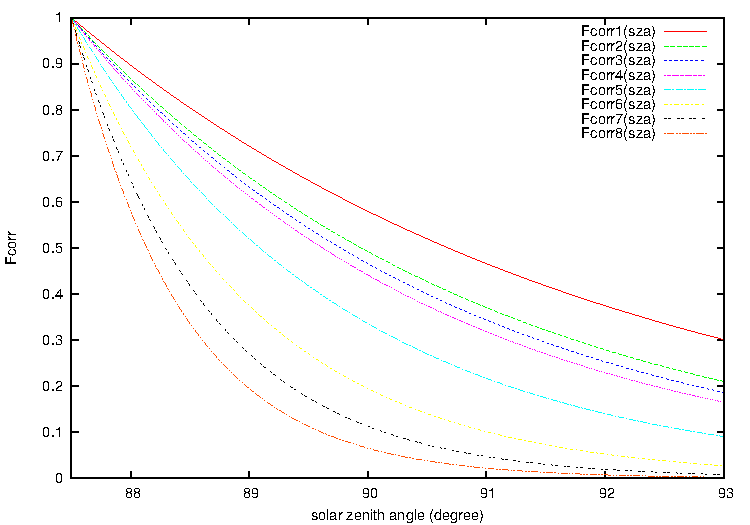
\includegraphics[width=\columnwidth]{lamago}
  \end{center}
  \caption{Correction factor for large solar zenith angles according to
    \citet{2642}.}
  \label{fig:lamago}
\end{figure}

\section{Modifying JVAL and JVPP}

\subsection{Adding a new photolysis reaction}

To add the photolysis of a new species (called ``XYZ'' here) to the
code, the following changes are necessary:

\begin{itemize}\nosep
\item Add the photolysis to \code{messy_cmn_photol_mem.f90}:
  \begin{itemize}\nosep
  \item add \code{ip_XYZ}
  \item increase \code{IP_MAX}
  \item add string to \code{jname}
  \end{itemize}
\item Create a new namelist file \code{XYZ.nml} with appropriate values
  and save it in the \code{dat_lit/spectra/} directory:
  \begin{itemize}
  \item define the MECCA equation tag \code{eqntag}
  \item define the reaction \code{texrxn} and a note with a reference
    \code{texnote} in La\TeX\ syntax
  \item if the default is not suitable, define \code{fj_corr} according
    to \citet{2642}
  \item if the default is not suitable, define the degree of the fitting
    functions \code{deg_tconst} and/or \code{deg_tdep}
  \item optionally, define \code{lya_ir} for a Lyman-$\alpha$ or
    infrared contribution
  \end{itemize}
\item Get the UV/VIS spectrum (e.g., from \citet{2872}) and enter it to
  a new file \code{XYZ.sig} in the \code{dat_lit/spectra/} directory.
\item If the cross sections are temperature-dependent, choose one of the
  following options:
  \begin{itemize}\nosep
  \item Create a \verb|XYZ.s2t| or \verb|XYZ.s3t| file if the spectrum
    is known at two or three temperatures, respectively.
  \item Create a \verb|XYZ.tc1|, \verb|XYZ.tc2|, or \verb|XYZ.tc3| file
    if the spectrum can be described with a function containing 1, 2, or
    3 parameters. Add the corresponding function to \verb|SUBROUTINE|
    \verb|calc_tdep| in \verb|jvpp_step2.f90|.
  \item For more complex cases, add an individual wavelength-dependent
    function at the end of \verb|SUBROUTINE| \verb|calc_tdep| in
    \verb|jvpp_step2.f90|.
  \end{itemize}
\item If the quantum yield is not always equal to one, add a
  \verb|XYZ.phi| file to the directory \code{dat_lit/spectra/}.
\item Execute the JVPP code via \verb|xjvpp| as described in
  Sect.~\ref{sec:execute}.
\item If the new photolysis reaction is used in the global ECHAM5/MESSy
  Atmospheric Chemistry (EMAC) model \citep{2400}, it is necessary to
  activate its calculation in \verb|messy_jval_si.f90| with:\\
  \verb|IF (TRIM(basename) == 'XYZ') &|
  \verb|  lps(ip_XYZ,j) = .TRUE.|
\end{itemize}

\subsection{Evaluating changes in JVPP}

To compare the spectra to those that were used in MESSy-1.7, go to the
directory \verb|workdir_jnl|, and run the (automatically generated)
ferret script \verb|jvpp_step1.jnl|. To check the quality of the
polynomial fits, run \verb|jvpp_step3_tconst.jnl| and
\verb|jvpp_step3_tdep.jnl| in the same directory. To check if the
temperature dependence of a spectrum was calculated correctly in step 2,
adjust and run \verb|jnl/tdep.jnl|.

\subsection{Evaluating changes in JVAL}

To evaluate how your modifications change the calculated $J$-values,
follow these steps:

\begin{itemize}\nosep
\item Run the JVAL column model via \verb|xjval| as described above.
\item Rename the resulting netcdf file, using a descriptive name, e.g.:\\
  \verb|mv jval.nc jval_BASE.nc|
\item Optionally, make a backup of the include file, using a descriptive
  name, e.g.:\\
  \verb|cp messy_jval_jvpp.inc|\\
  \verb|   messy_jval_jvpp_BASE.inc|
\item Modify the JVPP code as desired and create a new include file via
  \verb|xjvpp|.
\item Run the JVAL column model again, then rename the output using a
  different name, e.g., ``\verb|NEW|'' instead of ``\verb|BASE|''.
\item Edit the ferret script \verb|compare_jval.jnl|:
  \begin{itemize}\nosep
  \item Select two netcdf files for the comparison, e.g.:\\
    \verb|USE "jval_BASE.nc"|\\
    \verb|USE "jval_NEW.nc"|
  \item Select one or more photolysis reactions for the comparison, e.g.:\\
    \verb|GO _compare_jval J_O3P|\\
    \verb|GO _compare_jval J_O1D|
  \end{itemize}
\item Execute the ferret script:\\
  \verb|ferret|\\ 
  \verb|go compare_jval.jnl|
\end{itemize}

\bibliographystyle{egu} % bst file
\bibliography{literat}  % bib files

\end{document}
